\section{Some generalities on Lie algebras}
    \subsection{Structure of finite-dimensional semi-simple Lie algebras}
        As a precursor to our main discussion, let us recall some features of the theory of finite-dimensional semi-simple Lie algebras, particularly about their structure.

        \begin{definition}[(Semi-)simple Lie algebras]
            A Lie algebra over an arbitrary commutative ring $k$ is said to be \textbf{simple} if and only if it admits no non-zero Lie ideals. A Lie algebra over $k$ is said to be \textbf{semi-simple} if and only if it is a direct sum of simple Lie algebras over $k$. 
        \end{definition}
        \begin{remark}
            As an easy consequence of the definition, semi-simple Lie algebras are centre-less. In this sense, they can be thought of as perfect Lie algebras with trivial centres. 
        \end{remark}

        Over a field $k$ that is algebraically closed and of characteristic $0$, much is known about the structure of a semi-simple Lie algebra $\g$ that is finite-dimensional when regarded as a $k$-vector space. The bulk of the content presented above is discussed in further details in any standard textbook on Lie algebras (cf. e.g. \cite{humphreys_lie_algebras} or the first half of \cite{carter_affine_lie_algebras}).

        Firsly, one of the most important features of finite-dimensional semi-simple Lie algebras (henceforth implicitly understood to be defined over a characteristic-$0$ and algebraically closed field $k$) is that each such Lie algebra posses an invariant and non-degenerate $k$-bilinear form which is unique up to $k^{\x}$-multiples. The canonical choice is the so-called Killing form, but in various other context, other natural choices such as the trace form are also very useful. 
        \begin{lemma}[The Killing form] \label{lemma: killing_form}
            Suppose that $\g$ is a finite-dimensional Lie algebra over an algebraically closed field $k$ of characteristic $0$ and write:
                $$\ad: \g \to \gl(\g)$$
            for the adjoint representation of $\g$. Define the \textbf{Killing\footnote{Named after Wilhelm Killing.} form} to be the symmetric $k$-bilinear form\footnote{... or equivalently, as a $k$-linear map $\kappa: \Sym^2_k(\g) \to k$.}:
                $$\kappa: \g \x \g \to k$$
            given by:
                $$\kappa(x, y) := \trace(\ad(x) \circ \ad(y))$$
            This bilinear form is $\g$-invariant, in the sense that:
                $$\forall x, y, z \in \g: \kappa([x, y], z) = \kappa(x, [y, z])$$
        \end{lemma}
        \begin{proposition}[Cartan's Semi-simplicity Criterion] \label{prop: cartan_semi_simplicity_criterion}
            Suppose that $\g$ is a finite-dimensional Lie algebra over an algebraically closed field $k$ of characteristic $0$. Then, $\g$ will be semi-simple if and only if the Killing form $\kappa$ is non-degenerate. 
        \end{proposition}
        \begin{example}[Failure of Cartan's Criterion over positive characteristics]
            The following example illustrates why it is crucial that we work over characteristic $0$ for the sequel to be valid.

            Let $p \not = 2$ be a prime and consider the Lie algebra $\sl_2(\F_p^{\alg})$, where by $\F_p^{\alg}/\F_p$, we mean a choice of algebraic closure. Suppose that we know that if $L$ is a Lie algebra then for every $x \in L$, the operator $[x, -]: L \to L$ is a derivation (recall that this is a consequence of the Jacobi identity in the definition of Lie algebras). This implies that for every $x \in \sl_2(\F_p^{\alg})$, the operator:
                $$\ad(x) := [x, -]$$
            is nilpotent, which in turn implies that the Killing form for $\sl_2(\F_p^{\alg})$ is $0$, as nilpotent matrices are of trace zero. At the same time, one can show easily that $\sl_2(\F_p^{\alg})$ is simple by identifying for it the basis:
                $$\left\{ \begin{pmatrix} 1 & 0 \\ 0 & -1 \end{pmatrix}, \begin{pmatrix} 0 & 1 \\ 0 & 0 \end{pmatrix}, \begin{pmatrix} 0 & 0 \\ 1 & 0 \end{pmatrix} \right\}$$
        \end{example}
        \begin{proposition}[Uniqueness of the Killing form] \label{prop: killing_form_uniqueness}
            Suppose that $\g$ is a finite-dimensional semi-simple Lie algebra over an algebraically closed field $k$ of characteristic $0$. If $\kappa'$ is any invariant and non-degenerate symmetric $k$-bilinear form on $\g$ then there will exist $c \in k^{\x}$ such that:
                $$\kappa' = c \kappa$$
        \end{proposition}

        Now, the existence and uniqueness (up to non-zero scalings) of a non-degenerate and invariant symmetric bilinear form allows us to construct a natural grading of any semi-simple Lie algebra by its \say{root lattice}, which is a certain finite free $\Z$-module of combinatorial origin. 
        \begin{definition}[Cartan subalgebras] \label{def: cartan_subalgebras}
            Suppose that $\g$ is a Lie algebra over an arbitrary field. A \textbf{Cartan subalgebra} of $\g$ is then a Lie subalgebra that is nilpotent and self-normalising.  
        \end{definition}
        \begin{remark}
            Suppose that $\g$ is a Lie algebra over an arbitrary field $k$. If:
                $$\dim_k \g < |k|$$
            then one is always guaranteed that $\g$ would admit Cartan subalgebras. In particular, any Lie algebra over a field of characteristic $0$ admits a Cartan subalgebra, as such fields have infinite cardinalities. 
        \end{remark}
        \begin{lemma}[Cartan subalgebras are maximal toral subalgebras] \label{lemma: cartan_subalgebras_are_maxaimal_toral_subalgebras}
            Suppose that $\g$ is a finite-dimensional semi-simple Lie algebra over an algebraically closed field $k$ of characteristic $0$. The set of Cartan subalgebras of $\g$ will then be the same as the set of maximal toral Lie subalgebras of $\g$ (i.e. a maximal abelian Lie subalgebra whose elements are semi-simple\footnote{This necessitates the algebraic closure assumption.} under the adjoint representation).  
        \end{lemma}
        \begin{lemma}[Cartan subalgebras are conjugate]
            Suppose that $\g$ is a finite-dimensional semi-simple Lie algebra over an algebraically closed field $k$ of characteristic $0$. Then, every Cartan subalgebra thereof is conjugate to one another, i.e. they are all isomorphic to one another, via inner automorphisms of $\g$. 
        \end{lemma}
        \begin{lemma}[Non-degeneracy of invariant bilinear forms on Cartan subalgebras] \label{lemma: non_degeneracy_of_invariant_bilinear_forms_on_cartan_subalgebras}
            Suppose that $\g$ is a finite-dimensional semi-simple Lie algebra over an algebraically closed field $k$ of characteristic $0$ and choose for it a Cartan subalgebra $\h$. Choose also a non-degenerate and invariant symmetric $k$-bilinear form $(-, -)_{\g}$ on $\g$, regarded as a $k$-linear map:
                $$(-, -)_{\g}: \Sym_k^2(\g) \to k$$
            Then, the domain restriction of this form to $\Sym_k^2(\h)$ remains non-degenerate. 
        \end{lemma}
        As such, when studying representations of representations of finite-dimensional semi-simple Lie algebras over algebraically closed fields of characteristic $0$, one can freely choose Cartan subalgebras and then work entirely with respect to that choice. 
        \begin{definition}[Weight spaces and root spaces]
            Suppose that $\g$ is a finite-dimensional semi-simple Lie algebra over an algebraically closed field $k$ of characteristic $0$, and choose for it a Cartan subalgebra $\h$. Let $V$ be a $\g$-module. Then, one can abstractly define the vector subspace of $V$ consisting of elements of \textbf{weight} $\mu \in \h^*$ to be:
                $$V[\mu] := \{v \in V \mid \forall h \in \h: h \cdot v = \mu(h) v\}$$
            The set of weights $\mu \in \h^*$ such that $V[\mu] \not \cong 0$ is denoted by $\Pi(V)$, and if:
                $$V \cong \bigoplus_{\mu \in \Pi(V)} V[\mu]$$
            then we will say that $V$ is a \textbf{weight module} for $\g$. 

            When $V \cong \g$ and carries the adjoint action of $\g$, we will instead refer to the non-zero weights as \textbf{roots}.
        \end{definition}
        \begin{theorem}[Root space decomposition for finite-dimensional semi-simple Lie algebras] \label{theorem: root_space_decomposition_for_finite_dimensional_semi_simple_lie_algebras}
            Suppose that $\g$ is a finite-dimensional semi-simple Lie algebra over an algebraically closed field $k$ of characteristic $0$, and choose for it a Cartan subalgebra $\h$. Then, under the adjoint action, $\g$ becomes a weight module over itself. Furthermore, for each $\alpha \in \Pi(\g) \setminus \{0\}$, one has that:
                $$\dim_k \g[\alpha] = 1$$
        \end{theorem}
        \begin{convention}
            Suppose that $\g$ is a finite-dimensional semi-simple Lie algebra over an algebraically closed field $k$ of characteristic $0$, choose for it a Cartan subalgebra, and let $\g$ act via the adjoint action on itself. Since Cartan subalgebras are abelian by definition, it is not hard to see that:
                $$\h \cong \g[0]$$
            and in light of this, one then often writes:
                $$\Phi := \Pi(\g) \setminus \{0\}$$
            to denote the set of roots of $\g$. The root space decomposition of $\g$ then takes the form:
                $$\g \cong \h \oplus \bigoplus_{\alpha \in \Phi} \g[\alpha]$$
        \end{convention}
        The following is a very useful and conceptual way to think about elements:
            $$x \in \g[\alpha]$$
        (i.e. \say{root vectors}). 
        \begin{lemma}[Action of root vectors]
            Suppose that $\g$ is a finite-dimensional semi-simple Lie algebra over an algebraically closed field $k$ of characteristic $0$ and choose for it a Cartan subalgebra $\h$. Let $V$ be an arbitrary $\g$-module. Then:
                $$\forall \alpha \in \Phi: \forall \mu \in \Pi(V): \g[\alpha] \cdot V[\mu] \subseteq V[\mu + \alpha]$$
        \end{lemma}
        Before we state an important corollary of this lemma, let us note that thanks to lemma \ref{lemma: non_degeneracy_of_invariant_bilinear_forms_on_cartan_subalgebras}, with respect to a choice of a Cartan subalgebra and a non-degenerate and invariant symmetric $k$-bilnear form on $\g$, one can canonically identify:
            $$\h \xrightarrow[]{\cong} \h^*$$
        via said bilinear form. 
        \begin{corollary}
            Suppose that $\g$ is a finite-dimensional semi-simple Lie algebra over an algebraically closed field $k$ of characteristic $0$ and choose for it a Cartan subalgebra $\h$. Choose also a non-degenerate and invariant symmetric $k$-bilinear form $(-, -)_{\g}$ on $\g$. For any given root:
                $$\alpha \in \Phi$$
            and corresponding root vectors $x_{\alpha} \in \g[\alpha], x_{\beta} \in \g[\beta]$, one has that:
                $$[x_{\alpha}, x_{-\alpha}] = (x_{\alpha}, x_{\beta})_{\g} \check{\alpha}$$
            where:
                $$\check{\alpha} \in \h$$
            is such that:
                $$(\alpha, \check{\alpha})_{\g} = 2$$
        \end{corollary}
        \begin{proposition}[Pairing of root spaces]
            Suppose that $\g$ is a finite-dimensional semi-simple Lie algebra over an algebraically closed field $k$ of characteristic $0$ and choose for it a Cartan subalgebra $\h$. Fix a non-degenerate and invariant symmetric $k$-bilinear form $(-, -)_{\g}$ on $\g$.
            \begin{enumerate}
                \item The set of roots $\Phi$ is a $k$-linear spanning subset of $\h^*$ (but it is \textit{not} $k$-linearly independent!).
                \item For a given pair of roots $\alpha, \beta \in \Phi$, one has that:
                    $$(\g[\alpha], \g[\beta])_{\g} \not = 0 \iff \alpha + \beta = 0$$
                Equivalently, one has that:
                    $$\forall \alpha \in \h^*: \alpha \in \Phi \iff -\alpha \in \Phi$$
                which shows that $\Phi$ is not $k$-linearly independent.
            \end{enumerate}
        \end{proposition}
        \begin{definition}[Simple roots, positive/negative roots; root systems]
            Suppose that $\g$ is a finite-dimensional semi-simple Lie algebra over an algebraically closed field $k$ of characteristic $0$ and choose for it a Cartan subalgebra $\h$. Fix a non-degenerate and invariant symmetric $k$-bilinear form $(-, -)_{\g}$ on $\g$.
            
            A \textit{choice} of a linearly independent subset of the set of roots $\Phi$ of $\g$ gives a set of \textbf{simple roots}. With respect to such a choice $\Phi^{\circ}$, one regards elements of $\Phi^+ := \Z_{> 0} \Phi^{\circ} \cap \Phi$ as \textbf{positive roots} and those of $\Phi^- := -\Phi^+$ as \textbf{negative roots}; simple roots are therefore positive by convention.

            The triple:
                $$(\h^*, \Phi, (-, -)_{\g})$$
            is a \textbf{root system} of $\g$, though typically only the set of roots $\Phi$ itself is referred to, as $\h$ (and hence $\h^*$) and $(-, -)_{\g}$ are fixed once and for all. 

            From a root system as above, one can also construct a \textbf{Cartan matrix}. By fixing an enumeration of simple roots:
                $$\Phi^{\circ} := \{\alpha_i\}_{1 \leq i \leq l}$$
            (with $l := \dim_k \h^*$), one can then construct an $l \x l$ matrix $C := (c_{ij})_{1 \leq i, j \leq l} \in \Mat_l(\Z)$ by setting:
                $$c_{ij} := (\alpha_i, \check{\alpha}_j)_{\g}$$
        \end{definition}
        \begin{remark}
            It is not hard to see that for every $\alpha \in \Phi$, if we write $s_{\alpha} \in \End_k(\h^*)$ for the operation of reflection about the hyperplane perpendicular to $k \alpha \subseteq \h^*$, then we will have that:
                $$s_{\alpha}(\Phi) \subseteq \Phi$$
        \end{remark}
        \begin{remark}[Dynkin diagrams]
            It is also not hard to show that the Cartan matrix associated to a root system is an instance of an adjacency matrix of an undirected graph. The graph in question is usually referred to as the \textbf{Dynkin diagram} of $\g$, and it is given by letting the set of vertices be in bijection with the set of simple roots, and the set of undirected edges between vertex $\alpha_i$ and $\alpha_j$, say, to be the integer $a_{ij} := 2 \delta_{ij} - c_{ij}$. From this fact, one can infer that $C$ is necessarily \textit{positive-definite}.

            Though it is less trivial of a task, it is nevertheless very well-known at this point that Dynkin diagrams attached to finite-dimensional simple Lie algebras over algebraically closed fields of characteristic $0$ are completely classifiable. There are $4$ \say{classical} families/types ($\sfA_l, \sfB_l, \sfC_l, \sfD_l$), and $3$ \say{exceptional} families/types ($\sfF_4, \sfG_2, \sfE_6, \sfE_7, \sfE_8$); among these, the types $\sfA_l, \sfD_l$, and $\sfE_6, \sfE_7, \sfE_8$ are said to be \say{simply laced} as between any two of their distinct vertices, there can be only at most one edge.
            \begin{figure}[H]
                \centering
                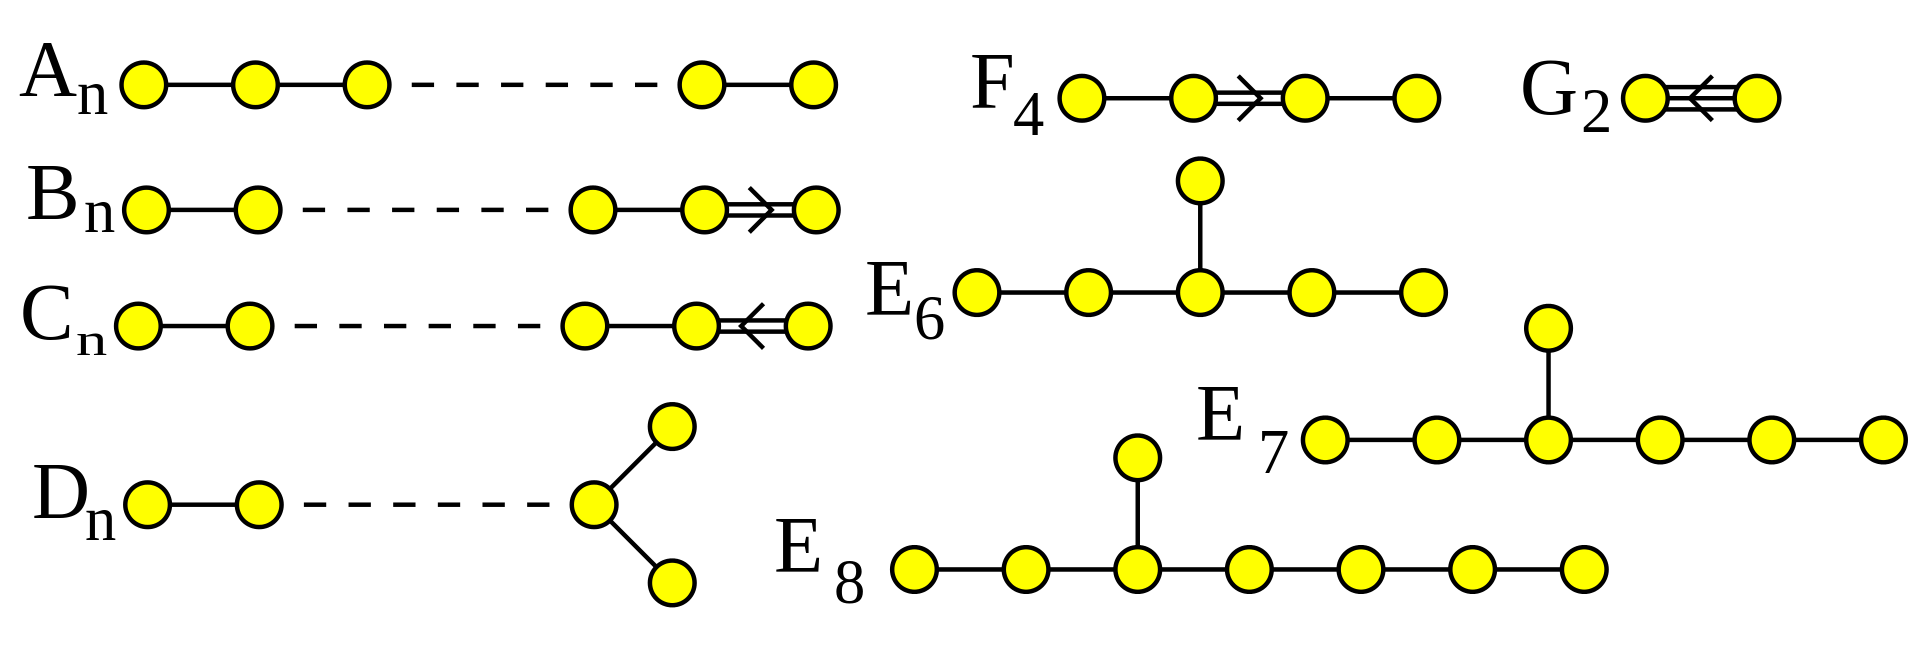
\includegraphics[width=0.5\linewidth]{Notes/Finite-dimensional simple Lie algebras/finite_type_dynkin_diagrams.png}
                \caption{Finite-type Dynkin diagrams}
                \label{fig: finite_type_dynkin_diagrams}
            \end{figure}
            
            An easy consequence of the construction of Dynkin diagrams from finite-dimensional semi-simple Lie algebras (one checks whether or not the associated Cartan matrix decomposes into a block sum of two submatrices along the diagonal) is that the function:
                $$\{ \text{Dynkin diagrams} \} \to \{ \text{finite-dimensional semi-simple Lie algebras over $k$} \}/\cong$$
            maps disjoint unions to direct sums and therefore, it suffices to ever only consider oneself with finite-dimensional simple Lie algebras. When a Dynkin diagram has only one connected component, we say that it is \textbf{connected}.
        \end{remark}
        The following result is a fundamental theorem in the study of finite-dimensional simple Lie algebras over algebraically closed fields of characteristic $0$. It essentially gives a bijective classification:
            $$\{ \text{connected Dynkin diagrams} \} \xrightarrow[]{\cong} \{ \text{finite-dimensional simple Lie algebras over $k$} \}/\cong$$
        which means that to give such a Lie algebra via a presentation by generators and relations is the same as giving its associated Cartan matrix. This is not only practically useful, but also is the mean by which one approaches Kac-Moody algebras, where the Cartan matrix is no longer required to be positive-definite (cf. \cite[Chapters 1-5]{kac_infinite_dimensional_lie_algebras}). 
        \begin{theorem}[Serre's Theorem]
            Let $\g$ be a finite-dimensional simple Lie algebra over an algebraically closed field of characteristic $0$ and denote its Cartan matrix by $(c_{ij})_{1 \leq i \leq l}$. Then, $\g$ is isomorphic to the Lie algebra generated by the set:
                $$\{h_i, e_i^{\pm}\}_{1 \leq i \leq l}$$
            whose elements are subjected to the following relations, given for all $1 \leq i, j \leq l$:
                $$[h_i, h_j] = 0$$
                $$[h_i, e_j^{\pm}] = \pm c_{ij} e_j^{\pm}, [e_i^+, e_j^-] = \delta_{ij} h_i$$
                $$\ad(e_i^{\pm})^{1 - c_{ij}}(e_j^{\pm}) = 0$$
            This is usually referred to as the \textbf{Chevalley-Serre} presentation for $\g$; final set of relations is usually known as the \textbf{Serre relations}.
        \end{theorem}
        \begin{corollary}
            For every root $\alpha \in \Phi$, any element $x \in \g[\alpha]$ is nilpotent under the vector representation of $\g$. 
        \end{corollary}
        \begin{corollary}[Triangular decomposition for finite-dimensional semi-simple Lie algebras]
            Let $\n^{\pm}$ denote the Lie subalgebras of $\g$ generated by the sets $\{e_i^{\pm}\}_{1 \leq i \leq l}$ respectively. Then:
                $$\g \cong \n^- \oplus \h \oplus \n^+$$
            This is usually called the \textbf{triangular decomposition} for $\g$. 
        \end{corollary}

        We end this subsection with a brief analysis of the easiest possible example of a finite-dimensional simple Lie algebra. 
        \begin{example}[$\sl_2$]
            Recall that $\sl_2(k)$ is the kernel of the trace map:
                $$\trace: \gl_2(k) \to k$$
            i.e. it is the Lie algebra of trace-zero $2 \x 2$-matrices whose Lie bracket is the usual commutator of matrices. It is of dimension $\dim_k \gl_2(k) - \dim_k k = 4 - 1 = 3$, and happens to be also generated by a set of cardinality $3$ (though this is a coincidence, due entirely to how \say{degenerate} of an example $\sl_2(k)$ is):
                $$\{h, e^+, e^-\}$$
            and the elements of this set are subjected to the relations:
                $$[h, e^{\pm}] = \pm 2 e^{\pm}, [e^+, e^-] = h$$
            One proves both of these statements by showing firstly that a basis for $\sl_2(k)$ is:
                $$\left\{ \begin{pmatrix} 1 & 0 \\ 0 & -1 \end{pmatrix}, \begin{pmatrix} 0 & 1 \\ 0 & 0 \end{pmatrix}, \begin{pmatrix} 0 & 0 \\ 1 & 0 \end{pmatrix} \right\}$$
            and then seeing that any Cartan subalgebra of $\sl_2(k)$ must therefore be isomorphic to $k \begin{pmatrix} 1 & 0 \\ 0 & -1 \end{pmatrix}$; the rest then follows. In particular, the Cartan matrix is just:
                $$\begin{pmatrix} 2 \end{pmatrix}$$
            and the Dynkin diagram consists of only a single vertex and no edges:
                $$\bullet$$
            From this, one gathers that $\sl_2(k)$ is of type $\sfA_1$. 
        \end{example}

    \subsection{Perfect Lie algebras and their central extensions}
        \begin{convention}
            We assume that the reader is familiar with basic homological algebra of modules over associative rings, and perhaps even the general abstract formulation of homological algebra in abelian categories, but we will not touch on derived categories. In particular, we assume familiarity with computations of Lie algebra cohomologies using Chevalley-Eilenberg resolutions. Furthermore, we assume that the reader is familiar with the interpretations of the low-dimensional cohomologies of a given Lie algebra (e.g. in terms of invariants, extensions, etc.).
        \end{convention}
    
        \begin{definition}[Extensions of modules]
            Let $R$ be an arbitrary associative ring. An \textbf{extension} of a left/right-$R$-module $M$ by another left/right-$R$-module $M'$ is a short exact sequence:
                $$
                    \begin{tikzcd}
                	0 & {M'} & E & M & 0
                	\arrow[from=1-1, to=1-2]
                	\arrow[tail, from=1-2, to=1-3]
                	\arrow[two heads, from=1-3, to=1-4]
                	\arrow[from=1-4, to=1-5]
                    \end{tikzcd}
                $$
            in the abelian category of left/right-$R$-modules. Such extensions form a natural category:
                $$\Ext_R^1(M, -)$$
            wherein the objects are extensions of $M$ some other left/right-$R$-module, and morphisms are morphisms of chain complexes whose component on $M$ is $\id_M$, e.g.:
                $$
                    \begin{tikzcd}
                	0 & {M_1} & {E_1} & M & 0 \\
                	0 & {M_2} & {E_2} & M & 0
                	\arrow[from=1-1, to=1-2]
                	\arrow[tail, from=1-2, to=1-3]
                	\arrow[two heads, from=1-3, to=1-4]
                	\arrow[from=1-4, to=1-5]
                	\arrow[from=2-1, to=2-2]
                	\arrow[tail, from=2-2, to=2-3]
                	\arrow[two heads, from=2-3, to=2-4]
                	\arrow[from=2-4, to=2-5]
                	\arrow["{}", from=1-2, to=2-2]
                	\arrow["{\id_M}", from=1-4, to=2-4]
                	\arrow[from=1-3, to=2-3]
                    \end{tikzcd}
                $$
                
            If $\Ext_R^1(M, -)$ admits initial objects, then those initial objects will be referred to as being \textbf{universal}. 

            An extension $0 \to M' \to E \xrightarrow[]{\pi} M \to 0$ is said to \textbf{split} if and only if $\pi$ has a section. Equivalently, if and only if $E \cong M \oplus M'$. 
        \end{definition}
        
        \begin{definition}[Extensions of Lie algebras]
            Let $k$ be a commutative ring and $\a$ be a Lie algebra over $k$. An \textbf{extension} of $\a$ by another Lie algebra $\z$ over $k$ is an extension of $k$-modules:
                $$0 \to \z \to \frake \to \a \to 0$$
            such that $\frake$ is also a Lie algebra over $k$. There is an obvious non-full subcategory of $\Ext^1_k(\a, -)$ spanned by Lie algebra extensions and morphisms of chain complexes of Lie algebras between them; we denote this category by $\Lie\Ext^1_k(\a, -)$. If this category admits initial objects, then those objects will be referred to as \textbf{universal extensions}.
            
            If:
                $$\z \subseteq \z(\frake)$$
            then we will say that the extension is \textbf{central}. The full subcategory of $\Lie\Ext^1_k(\a, -)$ spanned by central extensions is denoted by $\Cent\Lie\Ext^1_k(\a, -)$. Universal \textit{central} extensions are especially interesting and as such deserves their own notation: as they are necessarily isomorphic to one another should they exist, let us collectively denote the universal central extensions (UCEs) of $\a$ by $\uce(\a)$.
        \end{definition}
        \begin{proposition}[$H^2_{\Lie}$ = extensions]
            \cite[Theorem VIII.3.3]{hilton_stammbach_homological_algebra} Suppose that $\a$ is a Lie algebra over a commutative ring $k$. Then, the isomorphism classes of Lie algebra extensions of $\a$ (regarded as a left-$\rmU(\a)$-module) by some left-$\rmU(\a)$-module $M$:
                $$\pi_0\Ob( \Cent\Lie\Ext^1_k(\a, M) )$$
            is in bijection with elements of\footnote{... understood to be computed using the Chevalley-Eilenberg complex.}:
                $$H^2_{\Lie}(\a, M) := \Ext^2_{{}^l\rmU(\a)\mod}(k, M)$$
            More explicitly, given an extension:
                $$0 \to M \to \frake \to \a \to 0$$
            then up to a choice of $2$-cocyle:
                $$\sigma \in H^2_{\Lie}(\a, M)$$
            the Lie bracket on $\frake$ will be given by:
                $$\forall X, Y \in \a: \forall m, m' \in M: [ (X, m), (Y, m') ]_{\frake} := [X, Y]_{\a} + ( m \cdot Y - m' \cdot Y + \sigma(X, Y) )$$
        \end{proposition}
        \begin{corollary}[Trivial cohomological coefficients = central extensions]
            The isomorphism classes of central extensions of $\a$ are parametrised bijectively by elements of $H^2_{\Lie}(\a, k)$.
        \end{corollary}
        \begin{example}[Semi-direct products of Lie algebras]
            Let $k$ be an arbitrary commutative ring. 
            
            Let $\d$ be a Lie $k$-algebra acting on another Lie $k$-algebra $\z$, i.e. let $\t$ be a $\d$-module that happens also to be a Lie algebra over $k$. The canonical extension of $\d$ by $\z$ corresponding to the element:
                $$0 \in H^2_{\Lie}(\d, \z)$$
            is known as the \textbf{semi-direct product} of $\d$ by $\z$, and commonly denoted by:
                $$\z \rtimes \d$$
            For the sake of completeness, let us note that the Lie bracket here is given by:
                $$\forall D, D' \in \d: \forall K, K' \in \z: [ (D, K), (D', K') ]_{\z \rtimes \d} := [D, D']_{\d} + ( D \cdot K' - D' \cdot K )$$
            
            Interestingly, semi-direct products are split extensions, in the sense that there is a section Lie algebra homomorphism $\d \to \t \rtimes_{\rho} \d$, given by $D \mapsto (0, D)$.
        \end{example}
        \begin{example}
            If $\g$ is a finite-dimensional simple Lie algebra over an algebraically closed field $k$ of characteristic $0$, then the category of finite-dimensional $k$-linear representations of $\g$ will be semi-simple, and therefore the injective dimension of $\g$ will be $0$, i.e.:
                $$\injdim(\g\mod^{\fd}) = 0$$
            This implies that every central Lie algebra extension of $\g$ by a finite-dimensional centre over $k$ is necessarily trivial. 
        \end{example}

        At this point, a natural question to pose is as follows.
        \begin{question}
            Which class of Lie algebras naturally admits UCEs ? 
        \end{question}
        The notion of \say{perfect} Lie algebras is defined precisely to provide a source of examples that would answer this question.
        \begin{definition}[Perfect Lie algebras]
            A Lie algebra over a commutative ring is said to be \textbf{perfect} if it is equal to its derived subalgebra. 
        \end{definition}
        \begin{example}
            Since semi-simple Lie algebras lack non-zero ideals by definition, they are perfect. 
        \end{example}
        \begin{example}
            Let $A$ be any commutative algebra over some base commutative ring $k$, and let $\g$ be a semi-simple Lie algebra over $k$. Endow the $k$-module $\g_A := \g \tensor_k A$ with the Lie bracket:
                $$\forall x, y \in \g: \forall f, g \in A: [x f, y g]_{\g_A} := [x, y]_{\g} fg$$
            Then, $\g_A$ will be perfect when regraded as a Lie algebra over $k$, precisely because $\g$ is semi-simple.
        \end{example}
        \begin{definition}[Covering Lie algebras]
            Suppose that:
                $$0 \to \z \to \frake \xrightarrow[]{\pi} \a \to 0$$
            is a central extension of Lie algebras over some base commutative ring $k$. If $\frake$ is perfect then we will call the Lie algebra epimorphism:
                $$\pi: \frake \to \a$$
            a \textbf{covering} or a \textbf{cover} of $\a$. 

            There is an evident full subcategory of $\Cent\Lie\Ext^1_k(\a, -)$ where the objects are coverings of $\a$. Let us denote it by $\Cov_k(\a)$
        \end{definition}
        \begin{proposition}[Perfect Lie algebras admit UCEs] \label{prop: perfect_lie_algebras_admit_UCEs}
            \cite[Lemma 1.10]{garland_arithmetics_of_loop_groups} If $k$ is a field and $\a$ is a perfect Lie algebra over $k$, then $\Cov_k(\a)$ will have initial objects. Any such object will be referred to as a \textbf{universal cover} of $\a$, but still typically denoted by $\uce(\a)$.
        \end{proposition}
        \begin{definition}[Simply connected Lie algebras]
            A Lie algebra $\a$ over a commutative ring $k$ is said to be \textbf{simply connected} if every object of $\Cent\Lie\Ext^1_k(\a, -)$ splits as a Lie algebra extension, i.e. given any such object:
                $$0 \to \z \to \frake \xrightarrow[]{\pi} \a \to 0$$
            there exists a Lie algebra homomorphism:
                $$\sigma: \a \to \frake$$
            such that:
                $$\pi \circ \sigma = \id_{\a}$$
        \end{definition}
        \begin{proposition}[UCEs are simply connected]
            \cite[Theorem 1.16]{garland_arithmetics_of_loop_groups} Suppose that $\a$ is a Lie algebra over a field $k$. An object $\fraku \in \Ob( \Cov_k(\a) )$ is then initial (i.e. a UCE of $\a$) if and only if it is simply connected. 
        \end{proposition}
        \begin{example}
            If $\g$ is a finite-dimensional simple Lie algebra over an algebraically closed field $k$ of characteristic $0$, then the category of finite-dimensional $k$-linear representations of $\g[t] := \g \tensor_k k[t]$ will in fact \textit{not} be semi-simple. This suggests that $\g[t]$ admits non-trivial central extensions and in fact, since it is perfect, it admits a UCE, which can be shown to be by a $1$-dimensional centre:
                $$\uce(\g[t]) := \g[t] \oplus \bbC c$$
            Clearly, there is also a section:
                $$\g[t] \to \g[t] \oplus \bbC c$$
            given by:
                $$X \mapsto (X, 0)$$
        \end{example}